\subsection{2D}
\begin{frame}
  \frametitle{Multiphysics simulation results (2D)}
  \begin{figure}
   \vspace{-0.1in}
   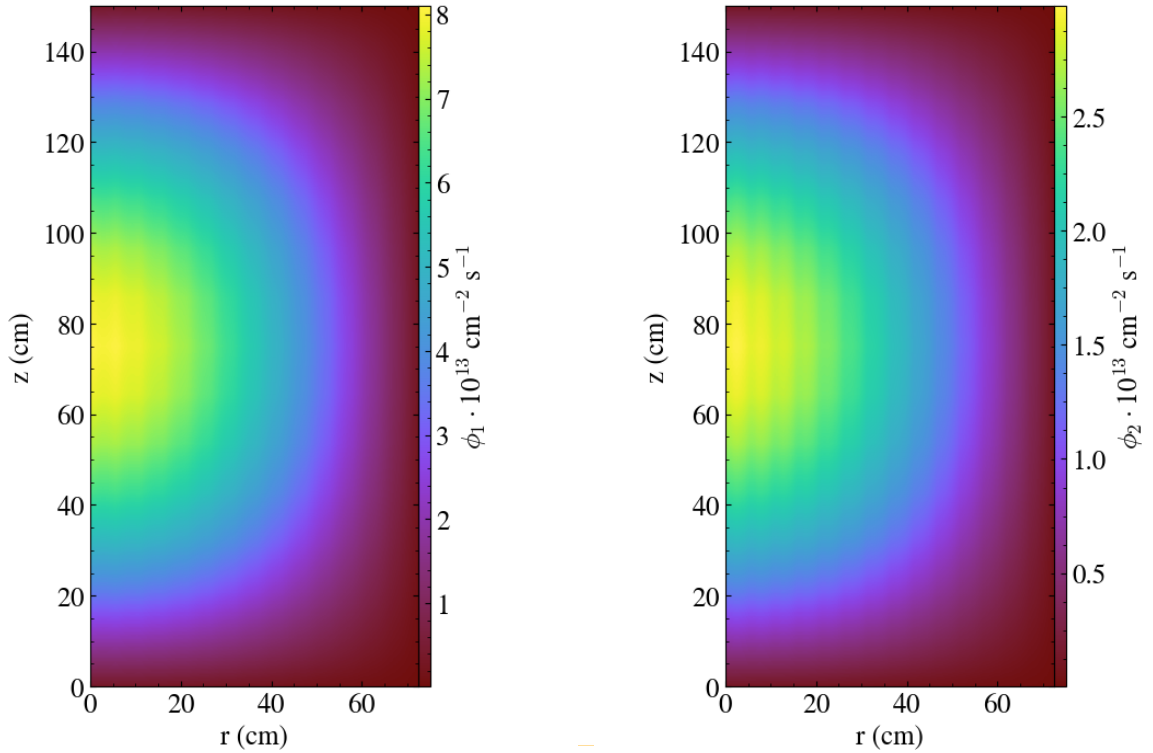
\includegraphics[height=0.85\textheight]{./images/moltres_flux.png}
   \vspace{-0.1in}
   \caption{Fast ($\phi_1$) and thermal ($\phi_2$) neutron flux obtained using Moltres 			\cite{lindsay_introduction_2018}.}
    \end{figure}
\end{frame}

\begin{frame}
  \frametitle{Multiphysics simulation results (2D) (2)}
  \begin{figure}[t]
   \vspace{-0.05in}
   \hspace*{-0.15in}
   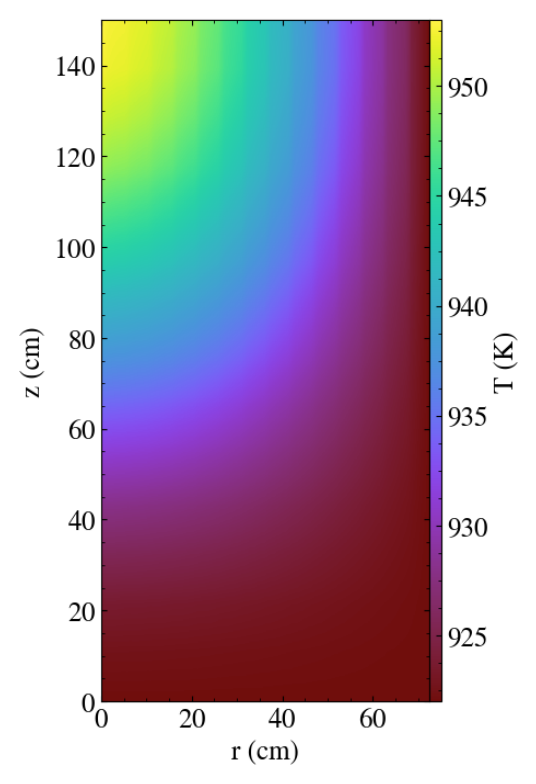
\includegraphics[height=0.85\textheight]{./images/moltres_temp.png}
   \vspace{-0.1in}
   \caption{Temperature in channel obtained using Moltres \cite{lindsay_introduction_2018}.}
    \end{figure}

\end{frame}

\begin{frame}
  \frametitle{Moltres vs MSRE Comparison}
  \begin{figure}[t]
   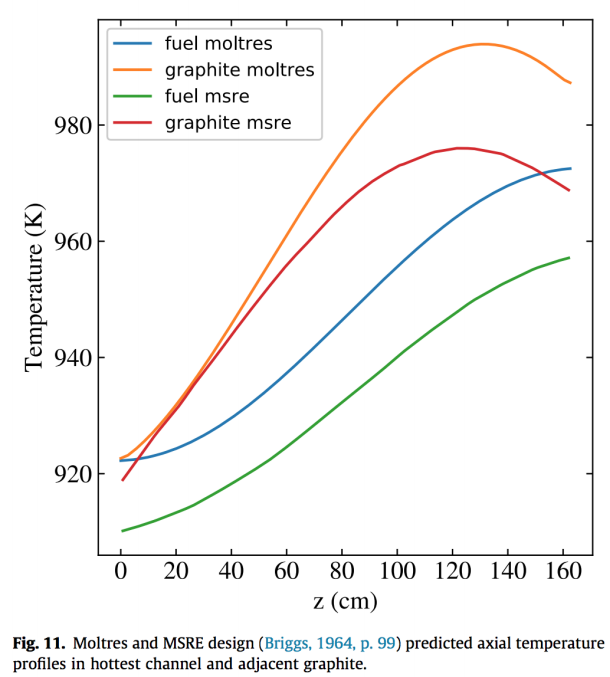
\includegraphics[height=0.85\textheight]{./images/msre_temp.png}
    \end{figure}

\end{frame}

\begin{frame}
  \frametitle{Moltres vs MSRE Comparison (2)}
  \begin{figure}[t]
   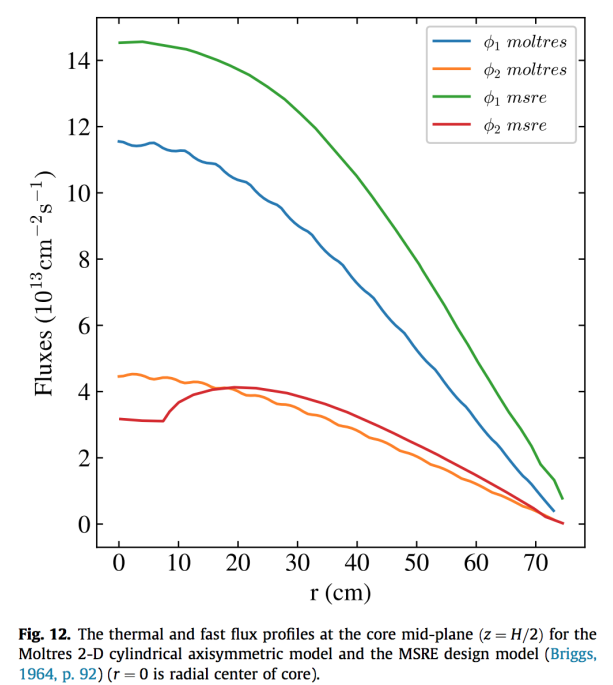
\includegraphics[height=0.85\textheight]{./images/msre_radial_flux.png}
    \end{figure}

\end{frame}

\begin{frame}
  \frametitle{Moltres vs MSRE Comparison (3)}
  \begin{figure}[t]
   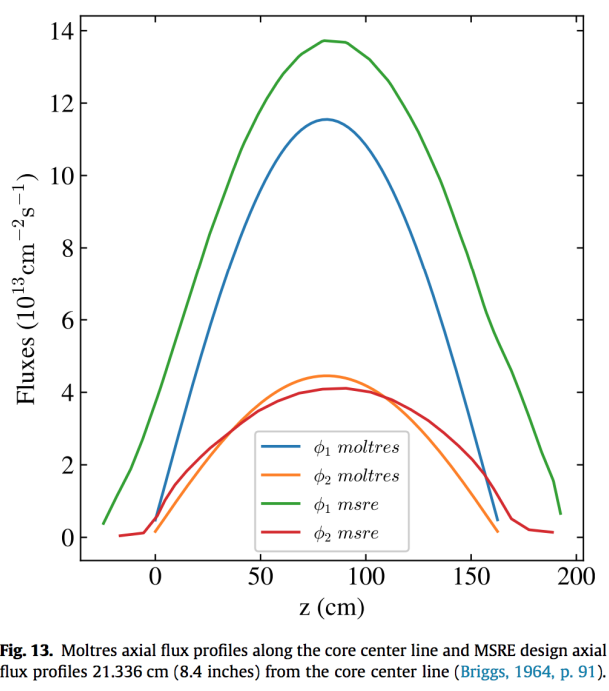
\includegraphics[height=0.85\textheight]{./images/msre_axial_flux.png}
    \end{figure}

\end{frame}

\subsection{3D}
\begin{frame}
  \frametitle{Multiphysics simulation results (3D)}
  \begin{figure}[t]
   \vspace{-0.15in}
   \hspace*{-0.8in}
   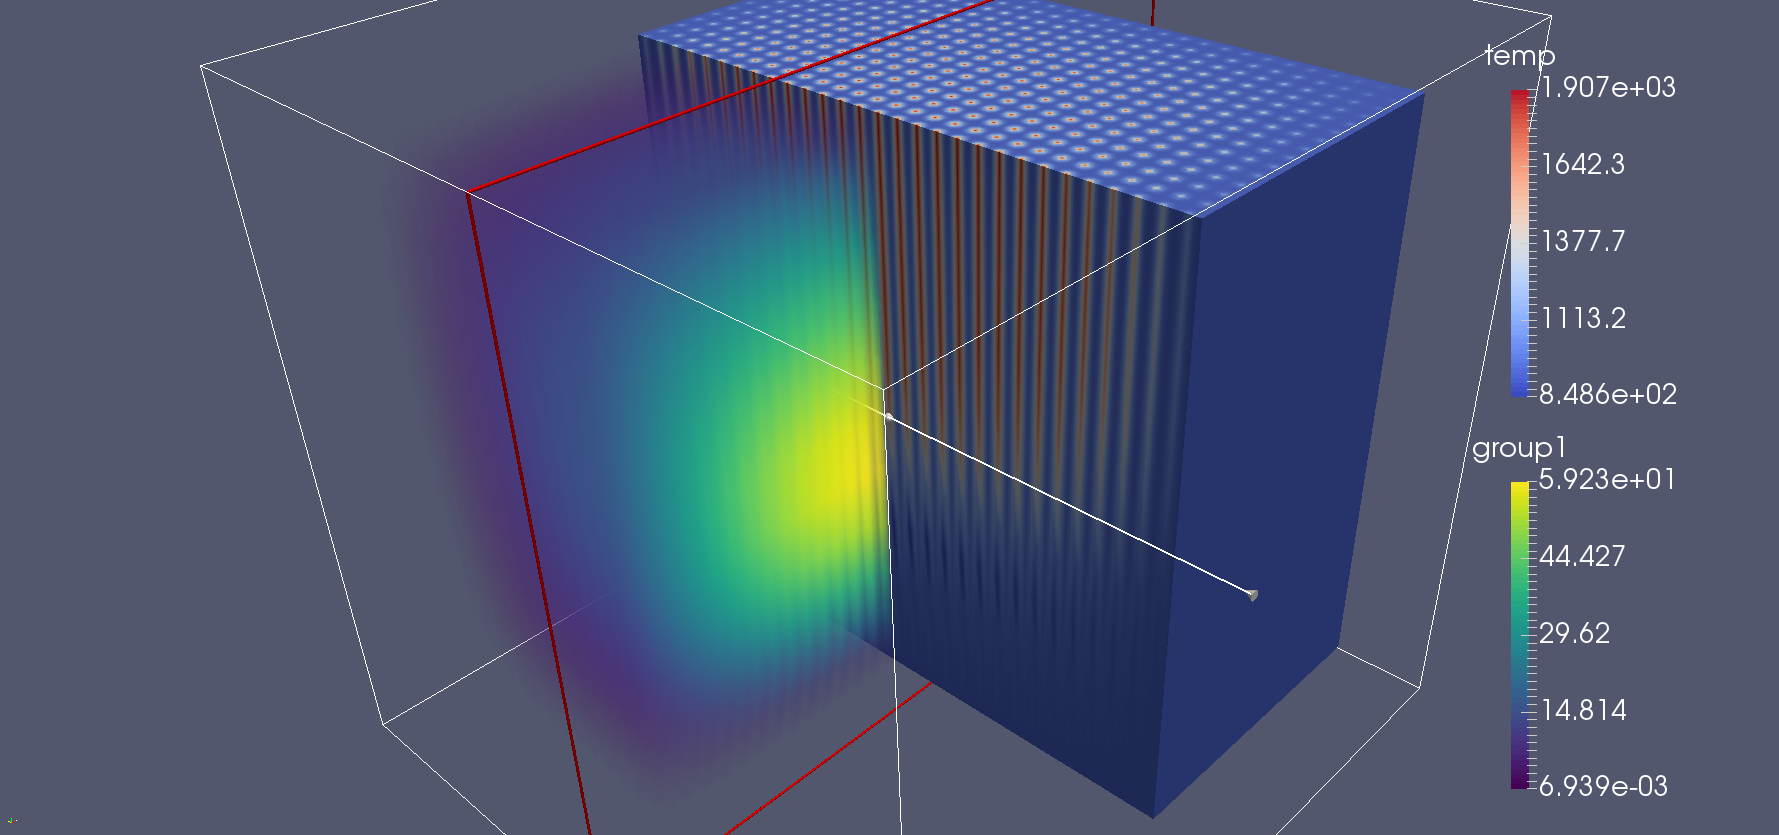
\includegraphics[height=0.8\textheight]{./images/moltres_3D.png}
   \caption{\gls{MSRE} steady-state temperature and fast neutron flux \cite{ridley_introduction_2017}.}
    \end{figure}
\end{frame}

\subsection{Scaling Studies}
\begin{frame}
        \frametitle{Scaling on Blue Waters}
Blue Waters:
         \begin{itemize}
                 \item XK7 nodes (two AMD 6276 Interlagos CPU per node
                 \item 16 floating-point bulldozer core units per node or 32 "integer" cores per node 
                 \item nominal clock speed is 2.45 GHz).
         \end{itemize}
\end{frame}

\begin{frame}
        \frametitle{Intra-Node Strong Scaling}
        \vspace*{-0.2in}
\begin{figure}[htpb]
  \centering
  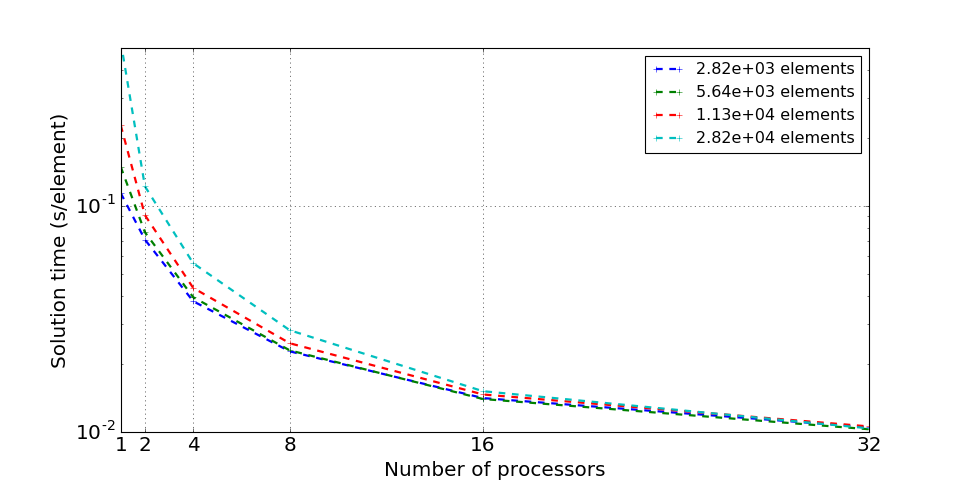
\includegraphics[width=\textwidth]{./images/intra-node_strong.png}
  \caption{Moltres intra-node strong scaling efficiency for various problem
        sizes, for $n_{cores} \in [1,32]$.  Up to 8 cores, larger problems required considerably more time per element because of cache overhead. However, beyond 8 cores, scaling demonstrates asymptotic dependence on the number of processors due to increasing communication costs. The best parallel efficiency for the intra-node study is approximately 89\%, achieved for the largest problem (28,200 elements).}
  \label{fig:intra_strong_scaling}
\end{figure}

\end{frame}

\begin{frame}
        \frametitle{Extra-node Strong Scaling}
        \vspace*{-0.2in}
\begin{figure}[htpb]
  \centering
  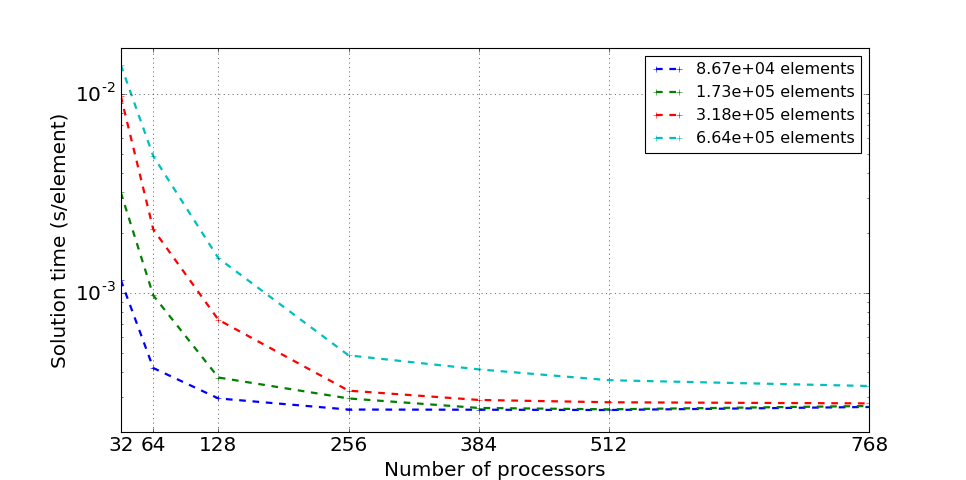
\includegraphics[width=\textwidth]{./images/extra-node_strong.png}
  \caption{Moltres extra-node strong scaling efficiency for various problem 
        sizes, for $n_{nodes} \in [1,24]$.  This takes into account 
        communication costs between nodes. Cache overhead causes performance 
        slow down for larger problems. Beyond 256 cores, simulation time per 
        element remains almost constant for small cases (86,655 and 173,310 
        elements) and slighly decreases for the two larger problems. Parallel 
        efficiency also grows with the problem size and reaches an optimal 
        value of 73\% for 664,355 elements.  }
  \label{fig:extra_strong_scaling}
\end{figure}

\end{frame}


\begin{frame}
        \frametitle{Intra-node Weak Scaling}
        \vspace*{-0.2in} 
\begin{figure}[htpb]
  \centering
  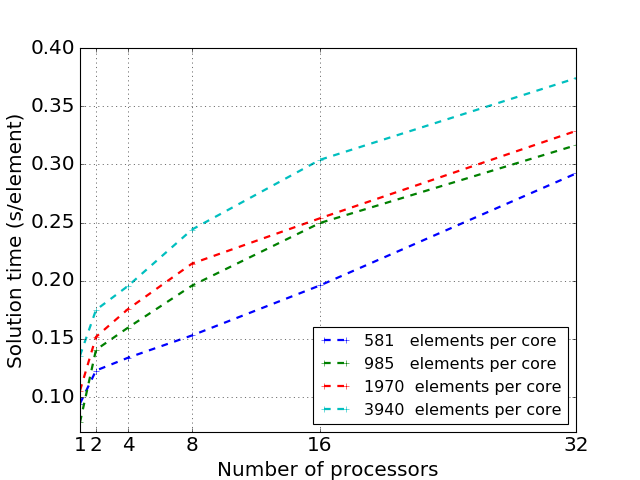
\includegraphics[width=0.7\textwidth]{./images/intra-node_weak.png}
  \caption{Weak scaling, in seconds per element vs. number of processors, for a constant number of elements
        per processor, and $n_{cores}\in[1,32]$.
        Largest drop in performance occurs when the number of cores increases 
        from one to $\approx$ 8, which corresponds to switching from no 
        communication to a 2-D domain decomposition.  Further reduction in performance of only about 50\% over a range of 32 cores is likely caused by increased communication latency appearing from collective \gls{MPI} calls.  
        }
  \label{fig:intra_weak}
\end{figure}
\end{frame}


\begin{frame}
\frametitle{Extra-node Weak Scaling}
        \vspace*{-0.2in}
\begin{figure}[htpb]
  \centering
  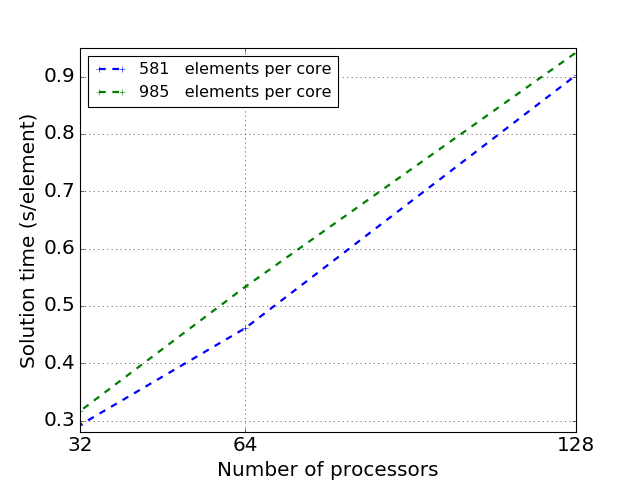
\includegraphics[width=0.75\textwidth]{./images/extra-node_weak.png}
  \caption{Weak scaling performance of Moltres on Blue Waters, in seconds per 
        element vs. number of processors, for a constant number of elements per processor and $n_{cores}\in[32,128]$.
        Performance drops by a factor of three, likely due to poor node 
        selection by the Blue Waters job scheduler, increased latency and bandwidth costs.
        }
  \label{fig:extra_weak}
\end{figure}
\end{frame}

\begin{frame}
        \frametitle{Scaling Conclusions}
        \begin{block}{Moltres scalability study results clearly indicate:}
        \begin{itemize} 
                \item Parallelization using LibMesh’s automatic domain 
                        decomposition is great, but not perfectly efficient.
                \item This scaling performance is satisfactory for MSR 
                        simulations approached thus far.
                \item Moltres is memory-bound and therefore very sensitive to host memory and memory bandwidth.
        \end{itemize}
        \end{block}
\end{frame}
%                         easured Moltres strong scaling with a simple 2D axisymmetric case for various problem sizes separately for intra-node (2,820; 5,640; 11,280 and 28,200 elements) and extra-node (86,655; 173,310; 317,735; 664,355 elements) setup on 

%\begin{frame}
%\includemedia[
%  activate=pageopen,
%  width=540pt,height=400pt,
%  addresource=./videos/test.mp4,
%  flashvars={%
%     source=./videos/test.mp4% same path as in addresource!
%   &autoPlay=true%    % optional configuration
%   &loop=true%        % variables
%  }  
%]{}{APlayer.swf}
%\end{frame}


